\documentclass[aspectratio=169,t,xcolor=table]{beamer}
\usepackage[utf8]{inputenc}

\usepackage{booktabs} 
\usepackage{subcaption}

\usetheme{Ufg}

\setbeamertemplate{theorems}[numbered]
\setbeamertemplate{caption}[numbered]

%-------------------------------------------------------------%
%----------------------- Primary Definitions -----------------%

% This command set the default Color, is also possible to choose a custom color
\setPrimaryColor{DarkGray} 

% First one is logo in title slide (we recommend use a horizontal image), and second one is the logo used in the remaining slides (we recommend use a square image)
\setLogos{lib/logos/valve_losgdg.pdf}{lib/logos/valve_logo.pdf} 


% -------------------------------------- Title Slide Information
\begin{document}
\title[Valve]{A year of ACO}
\subtitle{from prototype to default}

\author{Timur Kristóf}
\date{2020}
%-----------------------The next statement creates the title page.
\frame[noframenumbering]{\titlepage}


%------------------------------------------------Slide 1
\setLayout{vertical} % This command define the layout. 'vertical' can be replace with 'horizontal', 'blank, 'mainpoint', 'titlepage'

\begin{frame}
    \frametitle{Table of Contents}
    \tableofcontents
\end{frame}

\section{Our ACO story}

%---------------------------------------------------------
\setLayout{mainpoint}
{
\usebackgroundtemplate{
    \begin{picture}(100,256)(0,0)
        \put(0,0){
            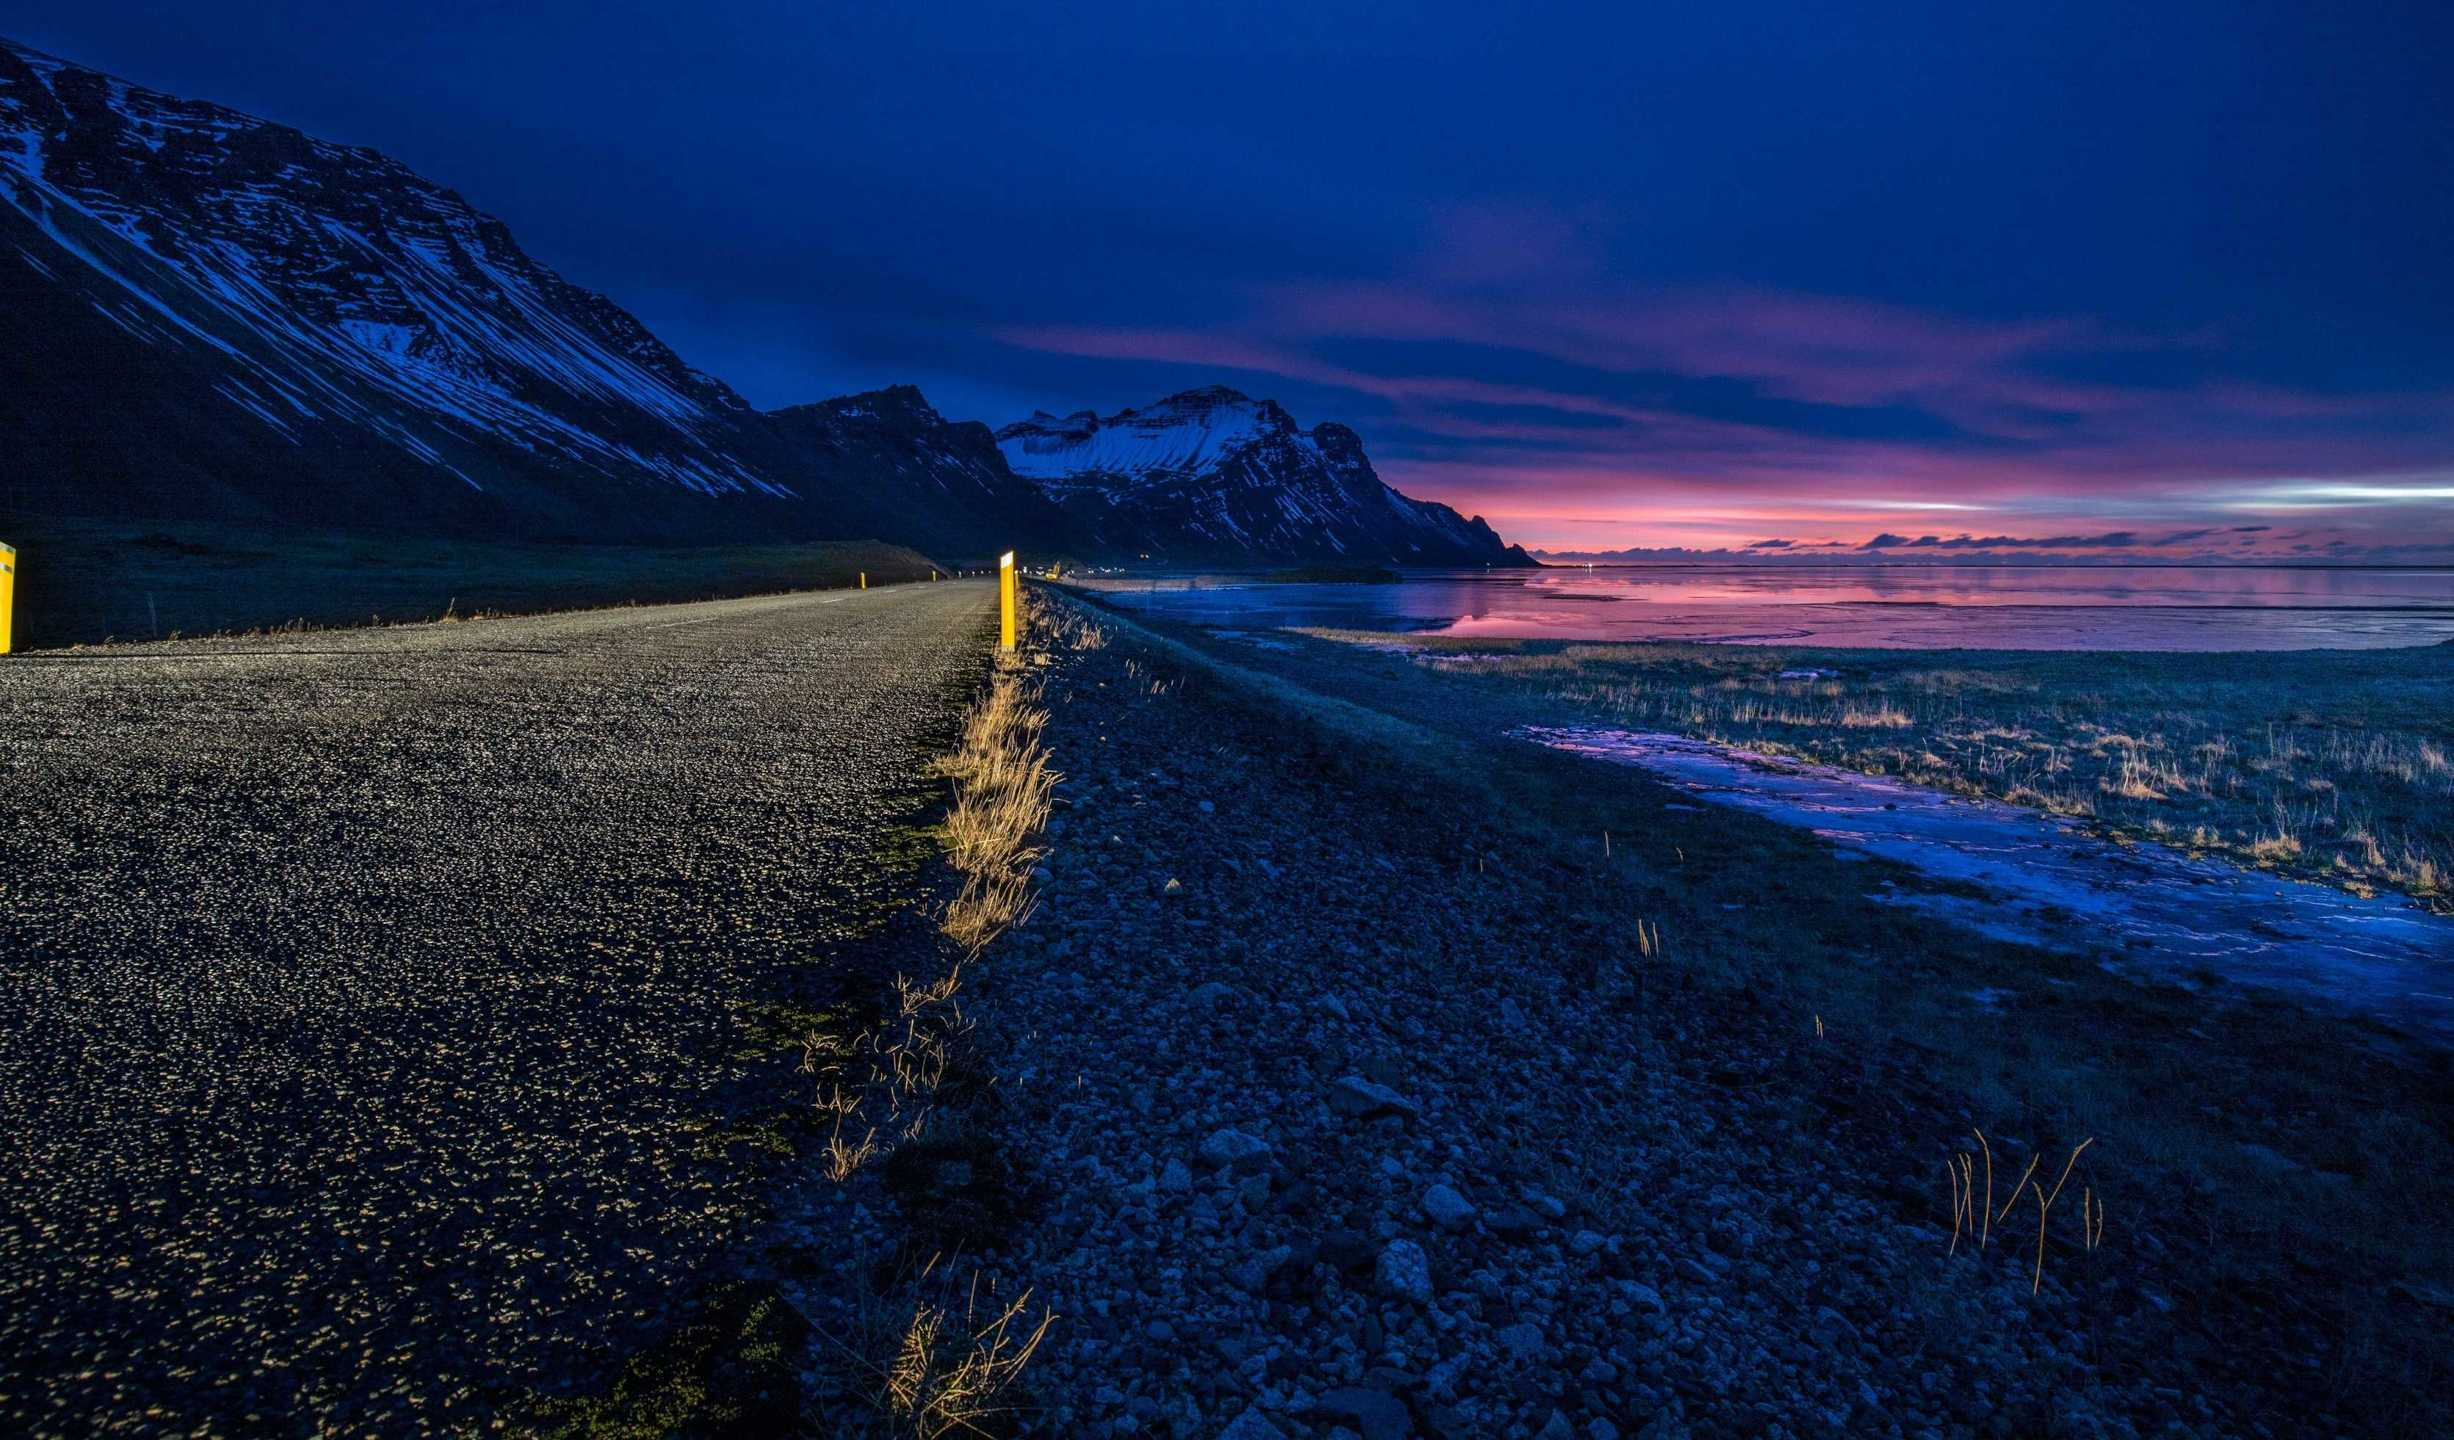
\includegraphics[width=\paperwidth]{figs/road.jpg}
        }
        % Put the frame title in the middle of page
        \put(160,115){
            \begin{tabular}{m{0.7\textwidth}}
                \begin{flushleft}
                   \selectfont \Huge \bfseries \insertframetitle
                \end{flushleft}
            \end{tabular}
        }
        \put(150,80){
            \begin{tikzpicture}
                \fill[white] (0,0) rectangle (0.2,3);
            \end{tikzpicture}
        }
        \put(20,20){\pgfuseimage{logo2_medium}}
    \end{picture}
}
\begin{frame}{Our ACO journey}
\end{frame}
}

%---------------------------------------------------------
\setLayout{vertical}
\begin{frame}{ACO motivation}

    \footnotesize

    \begin{block}{Fluid gaming}
        We'd like to give gamers a smooth, stutter-free experience, so we prioritize compilation speed.
    \end{block}

    \begin{block}{Developed in mesa}
        Issues can be fixed within mesa releases, independently of the schedule of other projects.
    \end{block}

    \begin{block}{Runtime performance}
        Good divergence analysis allows us to better optimize runtime performance.
    \end{block}

\end{frame}

%---------------------------------------------------------
\setLayout{mainpoint}
\begin{frame}{}
    \frametitle{Where we were last XDC}
\end{frame}

%---------------------------------------------------------
\setLayout{vertical}
\begin{frame}{Supported stages @ XDC 2019}

    \LARGE
    Started with PS only. \\
    Then added CS and VS.

\end{frame}

%---------------------------------------------------------
\setLayout{vertical}
\begin{frame}{Supported hardware @ XDC 2019}

    \LARGE
    Started on Polaris (GFX8) \\
    Then Vega was added (GFX9)

\end{frame}

%---------------------------------------------------------
\setLayout{vertical}
\begin{frame}{ACO 2019-2020 by numbers}

    \LARGE
    300+ merge requests \\
    5 current contributors \\
    15 supported shader stages \\
    5 supported HW generations (all GCN/RDNA) \\
    \ \\
    \normalsize
    Full feature parity
    \LARGE
    \begin{itemize}
    	\item VK exts supported by RADV work with ACO
    	\item Full conformance on newer HW
    \end{itemize}

\end{frame}

%---------------------------------------------------------
\setLayout{vertical}
\begin{frame}{No benchmarks this time, but...}

    \normalsize
    Runtime: \\
    \LARGE
    Phoronix has awesome benchmarks. \\
    \ \\
    \normalsize
    Compile time: \\
    \LARGE
    Consistent with what was shown in XDC2019.

\end{frame}

\section{How ACO works}

%---------------------------------------------------------
\setLayout{mainpoint}
\begin{frame}{}
    \frametitle{Where ACO fits in}
\end{frame}

%---------------------------------------------------------
\setLayout{vertical}
\begin{frame}{RADV/ACO shader compilation}

    \footnotesize

    \begin{alertblock}{SPIR-V to NIR}
        Parse the SPIR-V shader into NIR.
    \end{alertblock}

    \begin{alertblock}{NIR lowering and optimization}
        Lower the IR to be suitable for consumption by RADV / ACO.
    \end{alertblock}

    \begin{exampleblock}{ACO shader compilation}
        Compile the shader into a program the HW can execute.
    \end{exampleblock}

\end{frame}

%---------------------------------------------------------
\setLayout{mainpoint}
\begin{frame}{}
    \frametitle{Recap: how ACO works}
\end{frame}

%---------------------------------------------------------
\setLayout{vertical}
\begin{frame}{ACO compilation phases 1-3}

    \footnotesize

    \begin{block}{1. Instruction selection}
        Based around the NIR divergence analysis, emits ACO IR which is SSA.
    \end{block}

    \begin{block}{2. Value numbering, optimization}
        Common subexpression elimination, constant propagation, instruction combining.
    \end{block}

    \begin{block}{3. Setup reductions, insert exec mask}
        Ensure reductions work. Add instructions that control SIMD lanes.
    \end{block}

\end{frame}

%---------------------------------------------------------
\setLayout{vertical}
\begin{frame}{ACO compilation phases 4-6}

    \footnotesize

    \begin{block}{4. Live variable analysis}
        Calculate register need, used for spilling and scheduling.
    \end{block}

    \begin{block}{5. Spilling}
        Lower to CSSA, then try to decrease register usage.
    \end{block}

    \begin{block}{6. Instruction Scheduling}
        Move loads as high up as possible.
    \end{block}

\end{frame}

%---------------------------------------------------------
\setLayout{vertical}
\begin{frame}{ACO compilation phases 7-9}

    \footnotesize

    \begin{block}{7. Register Allocation}
        Works on SSA, emits shuffle code.
    \end{block}

    \begin{block}{8. SSA Elimination}
        Insert copies to match phi node semantics.
    \end{block}

    \begin{block}{9. Lower to HW instructions}
        Replace pseudo instructions with machine instructions.
    \end{block}

\end{frame}

%---------------------------------------------------------
\setLayout{vertical}
\begin{frame}{ACO compilation phases 10-11}

    \footnotesize

    \begin{block}{10. Insert wait states and NOPs, resolve hazards}
        Ensure correct behaviour of memory instructions, eliminate HW hazards.
    \end{block}

    \begin{block}{11. Assembler}
        ACO IR is already almost GCN/RDNA ASM, so only need to encode.
    \end{block}

\end{frame}

\section{Changes to ACO so that it can be the default compiler in RADV}

%---------------------------------------------------------
\setLayout{mainpoint}
\begin{frame}{}
    \frametitle{How we had to change it to make it the default}
\end{frame}

\subsection{New hardware support}

%---------------------------------------------------------
\setLayout{horizontal}
\begin{frame}{New hardware support}
\end{frame}

%---------------------------------------------------------
\setLayout{horizontal}
\begin{frame}{New (to us) hardware support}
    \normalsize
    \begin{table}[]
        \centering
        
        \renewcommand{\arraystretch}{1.5}
        \setlength{\tabcolsep}{10pt}
        
        {\rowcolors{2}{}{LightGray!10}
            \begin{tabular}{ p{2cm}p{8cm}p{2.5cm}  }
                \toprule 
                \textbf{Generation} & \textbf{Code names} & \textbf{Year} \\
                \midrule
                GFX6 & Pitcairn, Oldand, etc & 2012 \\
                GFX7 & Hawaii, Bonaire, etc & 2013 \\
                GFX10 & Navi & 2019 \\
                \bottomrule
            \end{tabular}
        }
    \end{table}
\end{frame}

%---------------------------------------------------------
\setLayout{horizontal}
\begin{frame}{New (to us) hardware support}
    \LARGE
    \begin{itemize}
        \item Different assembly encodings
        \item Some instructions missing on old HW \\
              or removed from new HW
        \item Missing subgroup features on old HW
        \item New (to us) hazards
        \item Very helpful community
    \end{itemize}
\end{frame}

\subsection{Small bitsizes}

%---------------------------------------------------------
\setLayout{horizontal}
\begin{frame}{Small bitsizes}
\end{frame}

%---------------------------------------------------------
\setLayout{horizontal}
\begin{frame}{Small bitsizes}
    \LARGE
    We had a lot of ideas.
\end{frame}

%---------------------------------------------------------
\setLayout{horizontal}
\begin{frame}{Small bitsizes}
    \LARGE
    We had a lot of \Huge\underline{bad} \LARGE ideas.
    \normalsize
    \ \\
    \ \\
    Lots of edge cases, more exceptions than rules.
\end{frame}

%---------------------------------------------------------
\setLayout{horizontal}
\begin{frame}{Small bitsizes}
    \LARGE
    Then we agreed to push the heavy lifting into RA, but...
\end{frame}

%---------------------------------------------------------
\setLayout{horizontal}
\begin{frame}{Small bitsizes}
    \LARGE
    Maintaining the register file \\
    \ \\
    \normalsize
    \begin{itemize}
        \item Previously: \\
              256 VGPRs + 106 SGPRs = 362 registers
        \item Now: \\
              We manage every byte of every register \\
              \ \\
              \footnotesize Yes, \large every \LARGE single \Huge byte.
    \end{itemize}
\end{frame}

%---------------------------------------------------------
\setLayout{horizontal}
\begin{frame}{Small bitsizes}
    \LARGE
    RA shuffles are now crazy \\
    \ \\
    \normalsize
    \begin{itemize}
        \item Previously: \\
              We had to move contents of registers
        \item Now: \\
              We move individual bytes between registers \\
              Sometimes even within the same register
    \end{itemize}
\end{frame}

%---------------------------------------------------------
\setLayout{horizontal}
\begin{frame}{Small bitsizes}
    \LARGE
    HW support is inconsistent \\
    \ \\
    \normalsize
    \begin{itemize}
        \item Some new HW: keeps high bits
        \item Other new HW: overwrites high bits
        \item Old HW: manual coding needed
    \end{itemize}
\end{frame}

\subsection{Geometry shaders}

%---------------------------------------------------------
\setLayout{horizontal}
\begin{frame}{Geometry shaders}
\end{frame}

%---------------------------------------------------------
\setLayout{horizontal}
\begin{frame}{Geometry shaders}
    \LARGE
    \begin{itemize}
        \item New intrinsics
        \item I/O: LDS, VRAM
        \item Figure out merged shaders
        \item GS copy shader
    \end{itemize}
\end{frame}

%---------------------------------------------------------
\setLayout{blank}
\begin{frame}{Geometry shaders: 4 new stages}
    \LARGE
    \begin{itemize}
        \item \texttt{vertex\_es} (GFX6-8)
        \item \texttt{geometry\_gs} (GFX6-8)
        \item \texttt{vertex\_geometry\_gs} (GFX9+)
        \item \texttt{gs\_copy\_vs}
    \end{itemize}
% The table is too complicated but not that important
%    \normalsize
%    \begin{table}[]
%        \centering
%        
%        \renewcommand{\arraystretch}{1.5}
%        \setlength{\tabcolsep}{10pt}
%        
%        {\rowcolors{2}{}{DarkGray!90}
%            \begin{tabular}{ p{3.5cm}p{1.5cm}p{1.5cm}p{1.5cm}p{1.5cm}  }
%                \toprule 
%                & SW VS & SW GS & (copy) & SW FS \\
%                \midrule
%                GFX6-8 only VS+PS & HW VS & - & - & HW PS \\
%                GFX6-8 with GS & \textcolor{red}{HW ES} & \textcolor{red}{HW GS} & \textcolor{red}{HW VS} & HW PS \\
%                \midrule
%                GFX9+ only VS+PS & HW VS & - & - & HW PS \\
%                GFX9+ with GS & \textcolor{red}{ESGS} & \textcolor{red}{ESGS} & \textcolor{red}{HW VS} & HW PS \\
%                \bottomrule
%            \end{tabular}
%        }
%    \end{table}
\end{frame}

%---------------------------------------------------------
\setLayout{blank}
\begin{frame}{Without geometry shaders: just VS}
    \footnotesize
    \underline{SW Vertex shader (HW VS):}
    \normalsize \texttt{\\
        VS go brrrr \\
        export to where PS can read from
    }
\end{frame}

%---------------------------------------------------------
\setLayout{blank}
\begin{frame}{Geometry shaders: separate stages}
    \footnotesize
    \underline{SW Vertex shader (HW ES):}
    \normalsize \texttt{\\
        VS go brrrr \\
        store outputs to VRAM
    }
    \footnotesize
    \ \\
    \ \\
    \underline{Geometry shader (HW GS):}
    \normalsize \texttt {\\
        load inputs from VRAM \\
        GS does its thing \\
        store outputs to VRAM
    }
    \footnotesize
    \ \\
    \ \\
    \underline{GS copy shader (HW VS):}
    \normalsize \texttt {\\
        load GS outputs from VRAM \\
        export to where PS can read from
    }
\end{frame}

%---------------------------------------------------------
\setLayout{blank}
\begin{frame}{Geometry shaders: merged VS+GS stage}
    \footnotesize \underline{SW VS+GS (HW GS):}
    \normalsize \texttt{\\
        if (am I a SW VS invocation?) \\
        ~~~~ VS go brrrr \\
        ~~~~ store outputs to LDS \\
        endif \\
        if (am I a SW GS invocation?) \\
        ~~~~ load inputs from LDS \\
        ~~~~ GS does its thing \\
        ~~~~ store outputs to VRAM \\
        endif
    }
    \footnotesize
    \ \\
    \ \\
    \underline{GS copy shader (HW VS):}
    \normalsize \texttt {\\
        load GS outputs from VRAM \\
        export to where PS can read from
    }
\end{frame}

%---------------------------------------------------------
\setLayout{blank}
\begin{frame}{Geometry shaders: GS copy shader}
    \normalsize
    Hardware limitations:
    \LARGE
    \begin{itemize}
        \item GS store their outputs in VRAM
        \item PS read their inputs from elsewhere
        \item So, we need to copy
    \end{itemize}
    \ \\
    \ \\
    \normalsize
    (These limitations are eliminated by NGG on Navi)
    
\end{frame}

\subsection{Tessellation}

%---------------------------------------------------------
\setLayout{horizontal}
\begin{frame}{Tessellation}
\end{frame}

%---------------------------------------------------------
\setLayout{horizontal}
\begin{frame}{Tessellation}
    \LARGE
    Tessellation shaders don't actually tessellate.
\end{frame}

%---------------------------------------------------------
\setLayout{horizontal}
\begin{frame}{Tessellation}
    \LARGE
    \begin{itemize}
        \item Lots of new intrinsics
        \item Lots of new stages
        \item Brain-twister I/O
    \end{itemize}
\end{frame}

%---------------------------------------------------------
\setLayout{horizontal}
\begin{frame}{Tessellation: merged stages}
    \normalsize
    On GFX9+: \\
    \LARGE
    VS and TCS are merged \\
    TES and GS are merged, too.
\end{frame}

%---------------------------------------------------------
\setLayout{blank}
\begin{frame}{Tessellation: 6 new stages}
    \normalsize
    When you have just tessellation:
    \LARGE
    \begin{itemize}
        \item VS: \texttt{vertex\_ls} (GFX6-8)
        \item TCS: \texttt{tess\_control\_hs} (GFX6-8)
        \item VS+TCS: \texttt{vertex\_tess\_control\_hs} (GFX9+)
        \item TES: \texttt{tess\_eval\_vs}
    \end{itemize}
    \normalsize
    \ \\
    \ \\
    When you also have GS:
    \LARGE
    \begin{itemize}
        \item TES: \texttt{tess\_eval\_es} (GFX6-8)
        \item TES+GS: \texttt{tess\_eval\_geometry\_gs} (GFX9+)
    \end{itemize}
%    \footnotesize
%    \begin{table}[]
%        \centering
%        
%        \renewcommand{\arraystretch}{1.5}
%        \setlength{\tabcolsep}{10pt}
%        
%        {\rowcolors{2}{}{DarkGray!90}
%            \begin{tabular}{ p{2.5cm}p{1.2cm}p{1.3cm}p{1.3cm}p{1.2cm}p{1.2cm}p{1.2cm} }
%                \toprule 
%                & SW VS & SW TCS & SW TES & SW GS & (copy) & SW FS \\
%                \midrule
%                GFX6-8 VS+PS & HW VS & - & - & - & - & HW PS \\
%                GFX6-8 w GS & HW ES & - & - & HW GS & HW VS & HW PS \\
%                GFX6-8 w tess & \textcolor{red}{HW LS} & \textcolor{red}{HW HS} & \textcolor{red}{HW VS} & - & - & HW PS \\
%                GFX6-8 w both & \textcolor{red}{HW LS} & \textcolor{red}{HW HS} & \textcolor{red}{HW ES} & HW GS & HW VS & HW PS \\
%                \midrule
%                GFX9+ VS+PS & HW VS & - & - & - & - & HW PS \\
%                GFX9+ w GS & ESGS & - & - & ESGS & HW VS & HW PS \\
%                GFX9+ w tess & \textcolor{red}{LSHS} & \textcolor{red}{LSHS} & \textcolor{red}{HW VS} & - & - & HW PS \\
%                GFX9+ w both & \textcolor{red}{LSHS} & \textcolor{red}{LSHS} & \textcolor{red}{ESGS} & \textcolor{red}{ESGS} & HW VS & HW PS \\
%                \bottomrule
%            \end{tabular}
%        }
%    \end{table}
\end{frame}

%---------------------------------------------------------
\setLayout{horizontal}
\begin{frame}{Tessellation: optimizing merged stages}
    \LARGE
    Sometimes the number of VS and TCS invocations are the same. \\
    \ \\
    \normalsize
    This happens when the input and output patch size are 3. \\
    Turns out they almost always are. \\
    In this case, VS outputs can be eliminated and transformed to temps.
\end{frame}

%---------------------------------------------------------
\setLayout{horizontal}
\begin{frame}{Tessellation: I/O}
    \LARGE
    Shaders can now read their own output. \\
    \ \\
    \normalsize
    So, sometimes we have to store them in both LDS and VRAM. \\
    Using different layouts.
\end{frame}

%---------------------------------------------------------
\setLayout{horizontal}
\begin{frame}{Wave32}
\end{frame}

%---------------------------------------------------------
\setLayout{horizontal}
\begin{frame}{Wave32}
    \normalsize
    Optionally, \\
    \LARGE
    you can have 32 SIMD lanes instead of 64 \\
    \ \\
    \normalsize
    This breaks a lot of assumptions we had.
\end{frame}

%---------------------------------------------------------
\setLayout{horizontal}
\begin{frame}{Wave32: special registers}
    \LARGE
    We had to change every usage of \texttt{exec} and \texttt{vcc}.
\end{frame}

%---------------------------------------------------------
\setLayout{horizontal}
\begin{frame}{Wave32: booleans}
    \normalsize
    Before: \\
    \LARGE
    Uniform (32-bit) vs. divergent (64-bit) \\
    \ \\
    \normalsize
    After: \\
    \LARGE
    All booleans are now per-lane \\
    Uniforms are optimized back
\end{frame}

%---------------------------------------------------------
\setLayout{horizontal}
\begin{frame}{Wave32: subgroups}
    \normalsize
    Subgroup size?
\end{frame}

%---------------------------------------------------------
\setLayout{horizontal}
\begin{frame}{Wave32: subgroups}
    \normalsize
    Subgroup size? \\
    \LARGE
    We always report 64 \\
    but pretend that 32 of those are disabled \\
    \ \\
    \normalsize
    Conforms to the spec, but still troublesome for naive, non-conformant apps \\
    eg. some expect to use the \texttt{(subgroup\_size - 1)}th lane
\end{frame}

%---------------------------------------------------------
\setLayout{horizontal}
\begin{frame}{Wave32: when to use?}
    \normalsize
    It's off by default (unless you use an env var) \\
    \LARGE
    CS: optionally available \\
    VS, TCS, TES, GS: decide based on divergence? \\
    PS: performs bad due to interpolation
\end{frame}

%---------------------------------------------------------
\setLayout{blank}
\begin{frame}{Btw, we fixed some bugs, too}
    \begin{columns}
        \column{0.5\textwidth}
        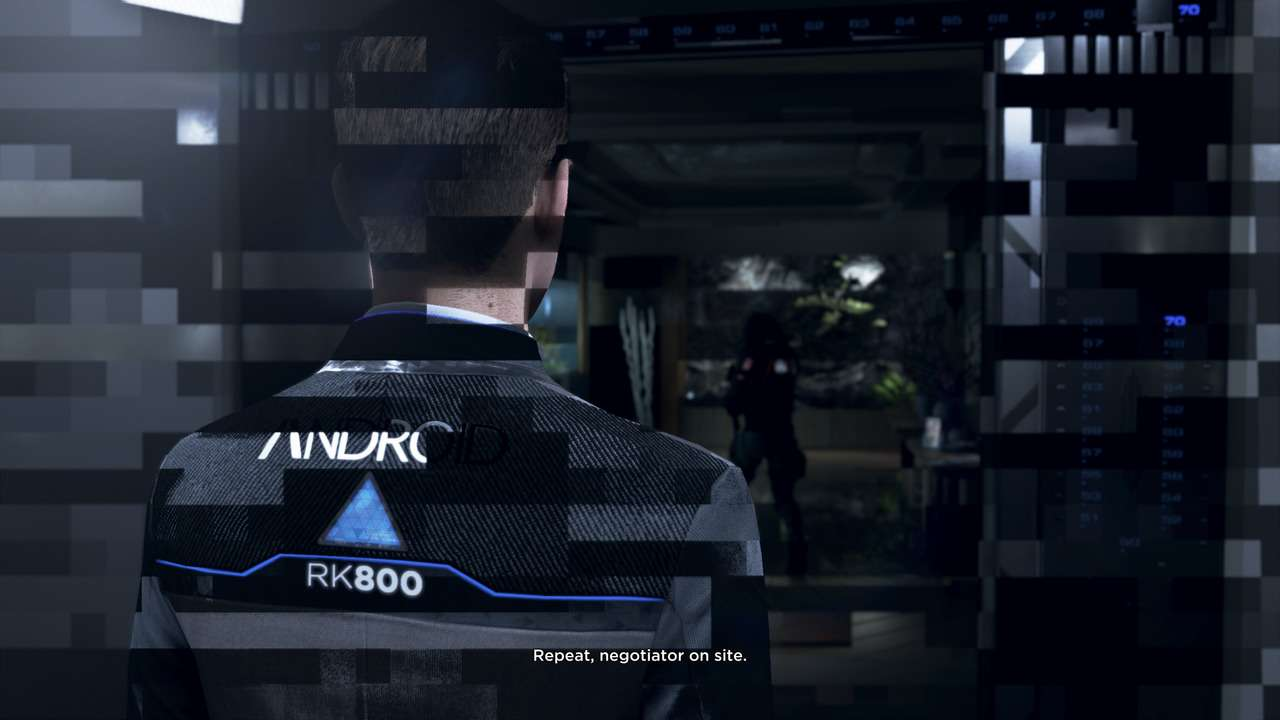
\includegraphics[height=3.2cm]{figs/bug1.jpg}
        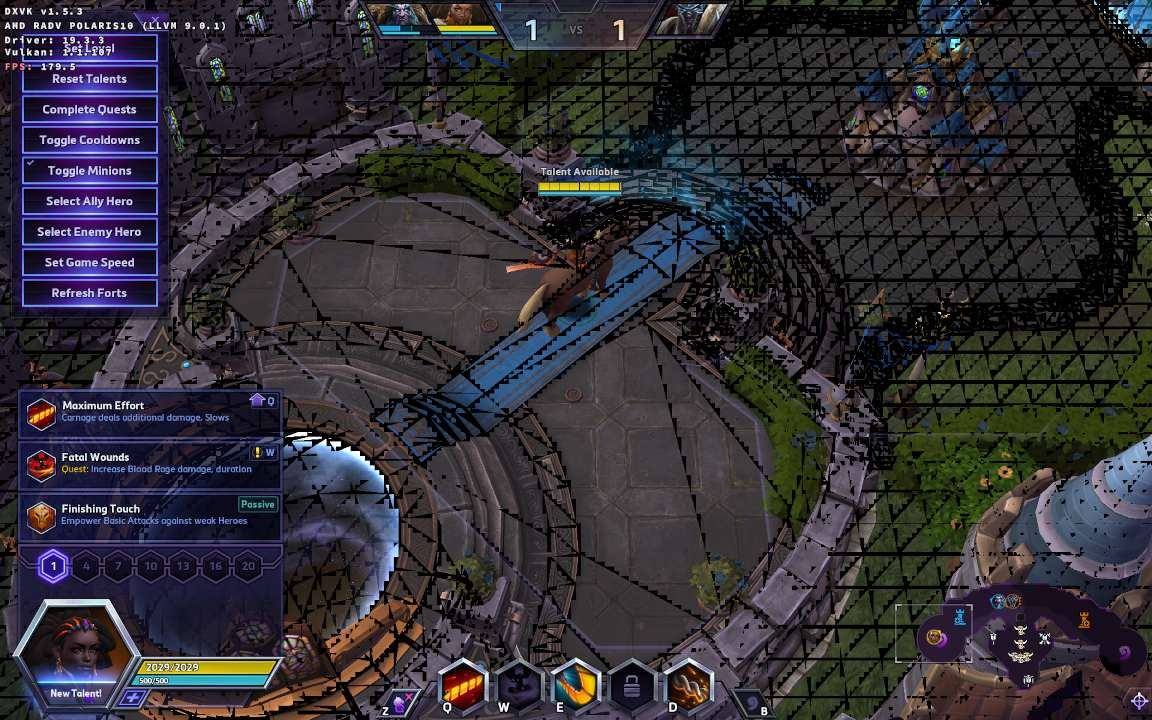
\includegraphics[height=3.2cm]{figs/bug2.jpg}

        \column{0.5\textwidth}
        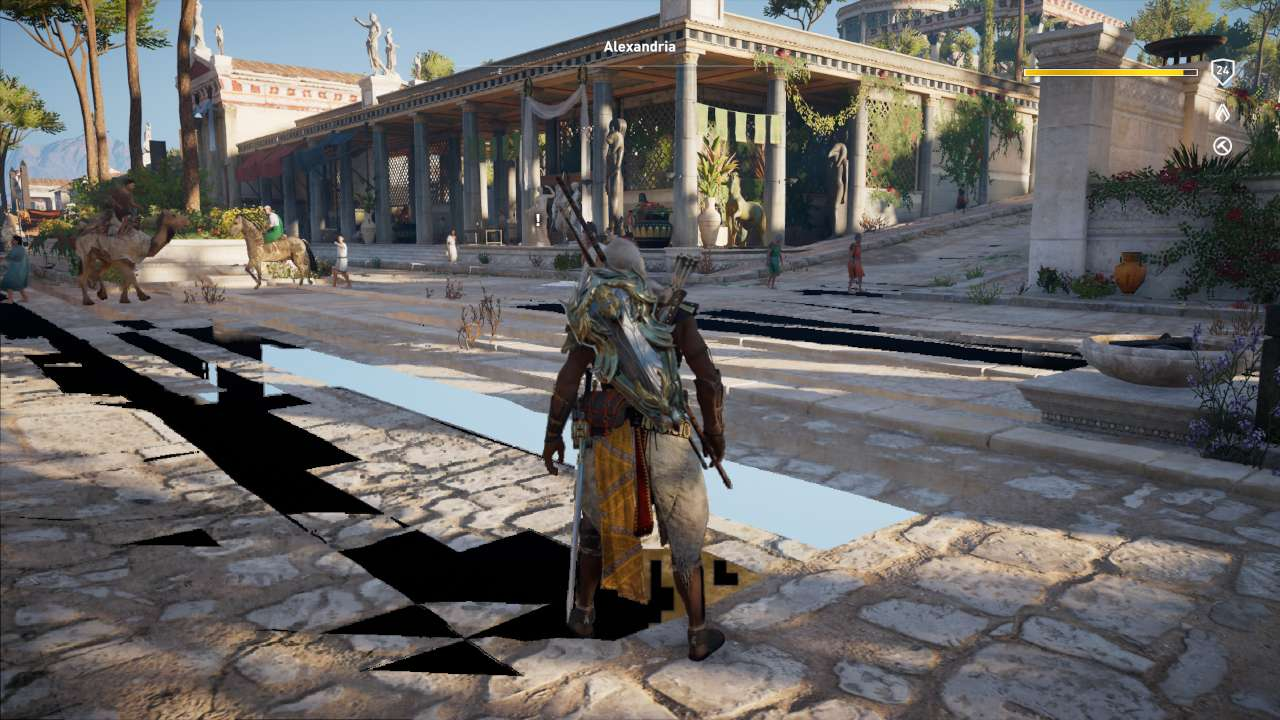
\includegraphics[height=3.2cm]{figs/bug3.jpg}
        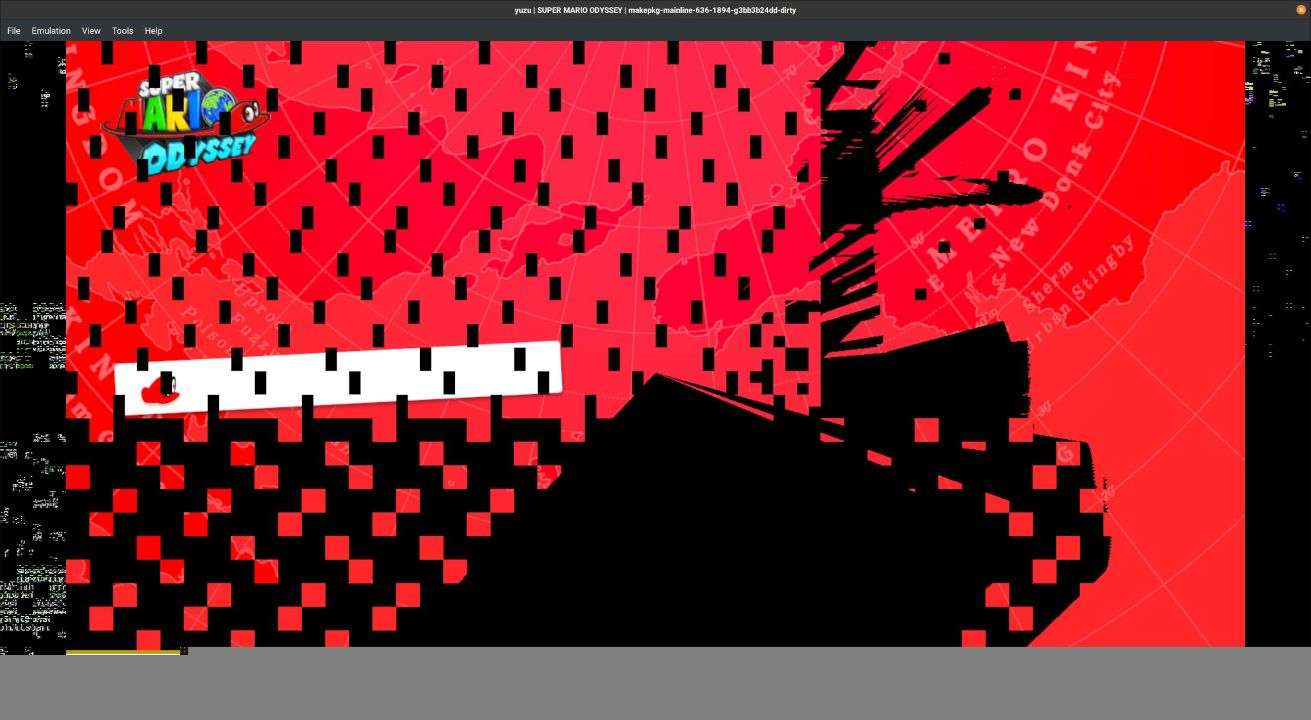
\includegraphics[height=3.2cm]{figs/bug4.jpg}
    \end{columns}
\end{frame}

%---------------------------------------------------------
\setLayout{blank}
\begin{frame}{Btw, we fixed some bugs, too}
    \LARGE
    And we added a unit testing framework to make sure they don't happen again.
\end{frame}

\section{Future plans}

%---------------------------------------------------------
\setLayout{mainpoint}
\begin{frame}{}
    \frametitle{Our plans for the future}
\end{frame}

%---------------------------------------------------------
\setLayout{horizontal}
\begin{frame}{RDNA 2 Support}
    \LARGE
    In progress
    \begin{itemize}
        \item We can look at RadeonSI
        \item We can browse LLVM code
    \end{itemize}
\end{frame}

%---------------------------------------------------------
\setLayout{horizontal}
\begin{frame}{RadeonSI (OpenGL) support}
    \LARGE
    Long road, but already started
    \begin{itemize}
        \item Unify shader arguments - Connor
        \item Unify I/O handling - Marek
        \item but ACO still depends on RADV internals
    \end{itemize}
\end{frame}

%---------------------------------------------------------
\setLayout{horizontal}
\begin{frame}{Ray Tracing}
    \LARGE
    \begin{itemize}
        \item There is a draft KHR extension
        \item And some LLVM code
        \item ...but no public RDNA 2 HW docs yet
    \end{itemize}
\end{frame}

%---------------------------------------------------------
\setLayout{horizontal}
\begin{frame}{Mesh shaders}
    \LARGE
    \begin{itemize}
        \item Possibly doable even on Navi 10 NGG
        \item ...but no KHR extension yet
    \end{itemize}
\end{frame}

%---------------------------------------------------------
\setLayout{horizontal}
\begin{frame}{More optimizations}
    \LARGE
    \begin{itemize}
        \item Rapid-packed math
    \end{itemize}
\end{frame}

%---------------------------------------------------------
\setLayout{horizontal}
\begin{frame}{More optimizations}
    \LARGE
    \begin{itemize}
        \item Clauses on Navi
        \item Post-RA scheduler
        \item NGG GS
        \item Others are also on the way
        \item And more
        \item And then some
    \end{itemize}
\end{frame}

%---------------------------------------------------------
\setLayout{blank}
{
    \usebackgroundtemplate{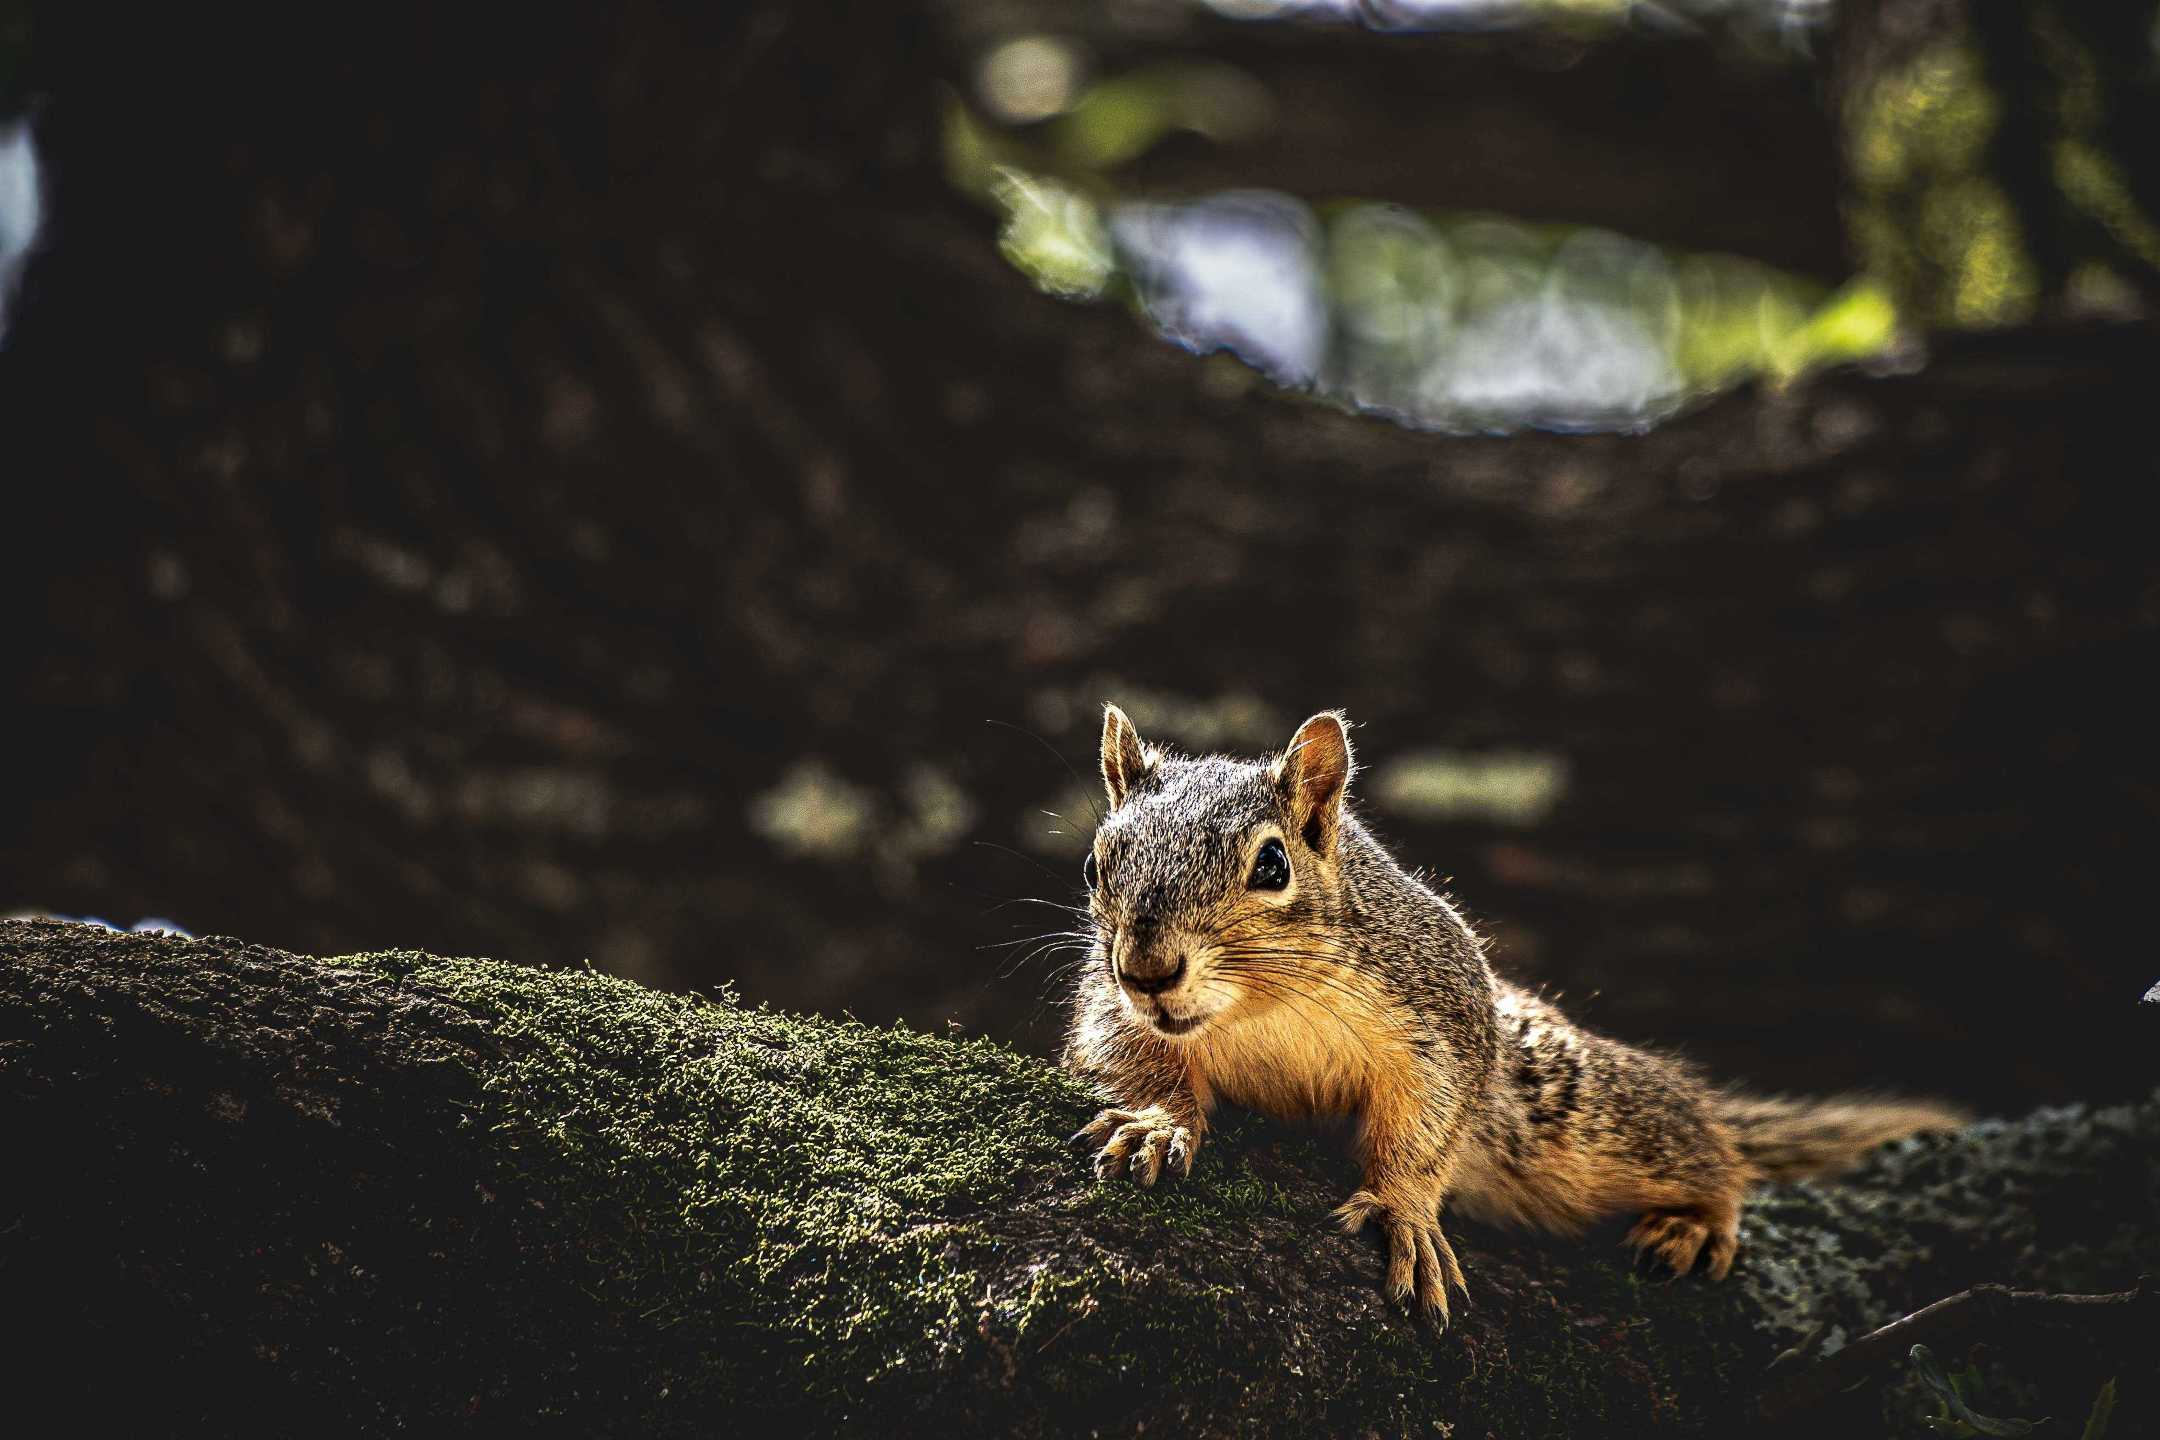
\includegraphics[width=\paperwidth]{figs/squirrel.jpg}}%
    \begin{frame}

        \vspace{2cm}
        
        \textbf{\Huge Thanks}
        
        \ \\
        
        \textbf{\LARGE Questions, suggestions, discussion?}
        
        \ \\
        
        \textbf{\normalsize A year of ACO}
        \ \\
        
        \text{\normalsize Timur Kristóf}
        
        \ \\
        
        \text{\footnotesize Venemo @ \#dri-devel, \#radeon, ...}
        \ \\
        \text{\footnotesize github.com/Venemo/xdc2020-aco}
        
        \vspace{1.4cm}
        
\includegraphics[height=1cm]{lib/logos/valve_logo.pdf}
        
    \end{frame}
}

%---------------------------------------------------------
\setLayout{titlepage}
\titlepage

\end{document}
